\documentclass[tikz,convert=pdf2svg]{standalone}
\usepackage{tikz}
\begin{document}
    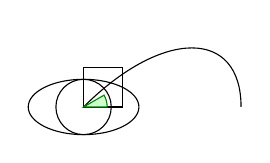
\begin{tikzpicture}
        \draw (0,0) circle (10pt);     %画一个圆心在原点,半径为10pt的圆;
        \draw (0,0) .. controls (1,1) and (2,1) .. (2,0);
        %画一个起点为(0,0),终点为(2,0),控制点为(1,1),(2,1)的贝塞尔曲线;
        \draw (0,0) ellipse (20pt and 10pt);       %画一个中心在原点,长轴、短轴分别为20pt和10pt的椭圆;
        \draw (0,0) rectangle (0.5,0.5);       %画一个从(0,0)到(0.5,0.5)的矩形
        \filldraw[fill=green!20!white, draw=green!50!black](0,0) -- (3mm,0mm) arc (0:30:3mm) -- cycle;
        %画一个扇形,并填充,扇形的边色和填充色的透明度不同。
    \end{tikzpicture}
\end{document}